\chapter{
  The LHC and CMS Experiment
 }\label{ch_cms}

The physics analysis is carried out using \gls{CMS} experiment at
\gls{CERN} \gls{LHC} accelerator. This chapter provides overview of \gls{LHC}
and detail of CMS experiment and its sub-detectors for particle tracking
and calorimetry.

\section{
  The Large Hadron Collider
 }\label{ch_cms:lhc}

The \gls{LHC} is the largest accelerator located at
\gls{CERN} in Geneva, Switzerland.
The main \gls{LHC} ring is 27\km{} in circumference
and around 50 to 175\m{} underground.
The \gls{LHC} is built to collide protons at 14\TeV{} center-of-mass energy,
LHC delivered proton-proton collisions at 7 and 8\TeV{}
during run-1 (2010--2012), and at 13\TeV{} center-of-mass energy during
run-2 (2015--2018)
~\cite{Evans:2008}.

The Figure~\ref{fig:lhc} describes \gls{CERN} accelerator complex.
The protons are sourced by ionizing hydrogen atoms
and then fed into \gls{LINAC}.
The \gls{LINAC} accelerates the protons to 50\MeV{} and sent to the booster.
Then the booster increases energy of protons to 1.4\GeV{} and
feeds it to the \gls{PS} which further increases energy to 25\GeV{}
and starts bunching them together with bunches 25\nanoseconds{} apart.
Then the proton bunches are passed through \gls{SPS} which increases energy
to 450\GeV{} and finally sent to main \gls{LHC} clockwise and counterclockwise
rings where they are accelerated to final energy required which is 6.5\TeV{}
for both bunches going clockwise and counterclockwise
to obtain collisions at 13\TeV{} center-of-mass energy.

The proton-proton collisions occurs at four different location where two
general purpose detectors \gls{CMS} and \gls{ATLAS}, and
two specific purpose detector \gls{ALICE} and \gls{LHCb} are located.

\begin{figure}[!ht]
  \centering
  \includegraphics[width=0.98\textwidth]{figures/lhc-scheme.png}
  \caption[A schematic of the CERN accelerator complex]%
  {A schematic of the CERN accelerator complex~\cite{image-lhc-scheme}}%
  \label{fig:lhc}
\end{figure}

\subsection{
  Integrated Luminosity
}\label{ch_cms:cms-lumi}

The number of events generated in a collisions for a given process is
\begin{equation}
  N = L \sigma
\end{equation}
where \(\sigma \) is cross-section of the process
and \(L\) is the luminosity of the \gls{LHC}.

\begin{figure}[!ht]
  \centering
  \includegraphics[width=0.5\textwidth]{figures/int_lumi_pp_run2.pdf}
  \caption[Cumulative delivered and recorded luminosity versus
    time for 2015--2018 proton-proton collisions]%
  {Cumulative delivered and recorded luminosity versus
    time for 2015--2018 proton-proton collisions~\cite{plot-cms-lumi}}%
  \label{fig:int-lumi}
\end{figure}

Cumulative luminosity delivered and recorded by \gls{CMS} during run-2 operation
in shown in Figure~\ref{fig:int-lumi}.
For run-2 standard physics analysis luminosity recorded during
2016--2018 is considered, and only runs certified as ``golden'' by \gls{CMS}
Luminosity \gls{POG} for analysis are used. The total luminosity for run-2
standard physics is 137.19\fbinv{}
and separately for years in Table~\ref{tab:years-lumi}
~\cite{CMS-PAS-LUM-17-001,CMS-PAS-LUM-17-004,CMS-PAS-LUM-18-002}.

\begin{table}[!ht]
  \centering
  \caption[Standard physics luminosity for run-2]%
  {Standard physics luminosity for run-2}
  \begin{tabular}{cccc}
    \toprule
    2016          & 2017          & 2018          & run-2          \\ \midrule
    35.92\fbinv{} & 41.53\fbinv{} & 59.74\fbinv{} & 137.19\fbinv{} \\
    \bottomrule
  \end{tabular}%
  \label{tab:years-lumi}
\end{table}

\section{
  The CMS Detector
 }\label{ch_cms:cms}

The \gls{CMS} detector is a general purpose detector.
A cutaway view of the detector is shown in Figure~\ref{fig:cms-cutaway}.
The detector is cylindrical with dimensions 21 meters long, and 15 meters
in diameter, and the whole detector weighs about 14000 tonnes.
The detector is built in slices with central region called ``barrel'',
and two closing end sides called ``endcap''.
A superconducting solenoid generates magnetic field of 3.8\Tesla{} inside
and 2\Tesla{} outside, and to contain the magnetic field outside of solenoid
and support structure of the detector massive steel yokes are used.This section
describes the subsystems of \gls{CMS} detector. For detailed technical
description refer to~\cite{CMS-JINST-S08004}.

\begin{figure}[!ht]
  \centering
  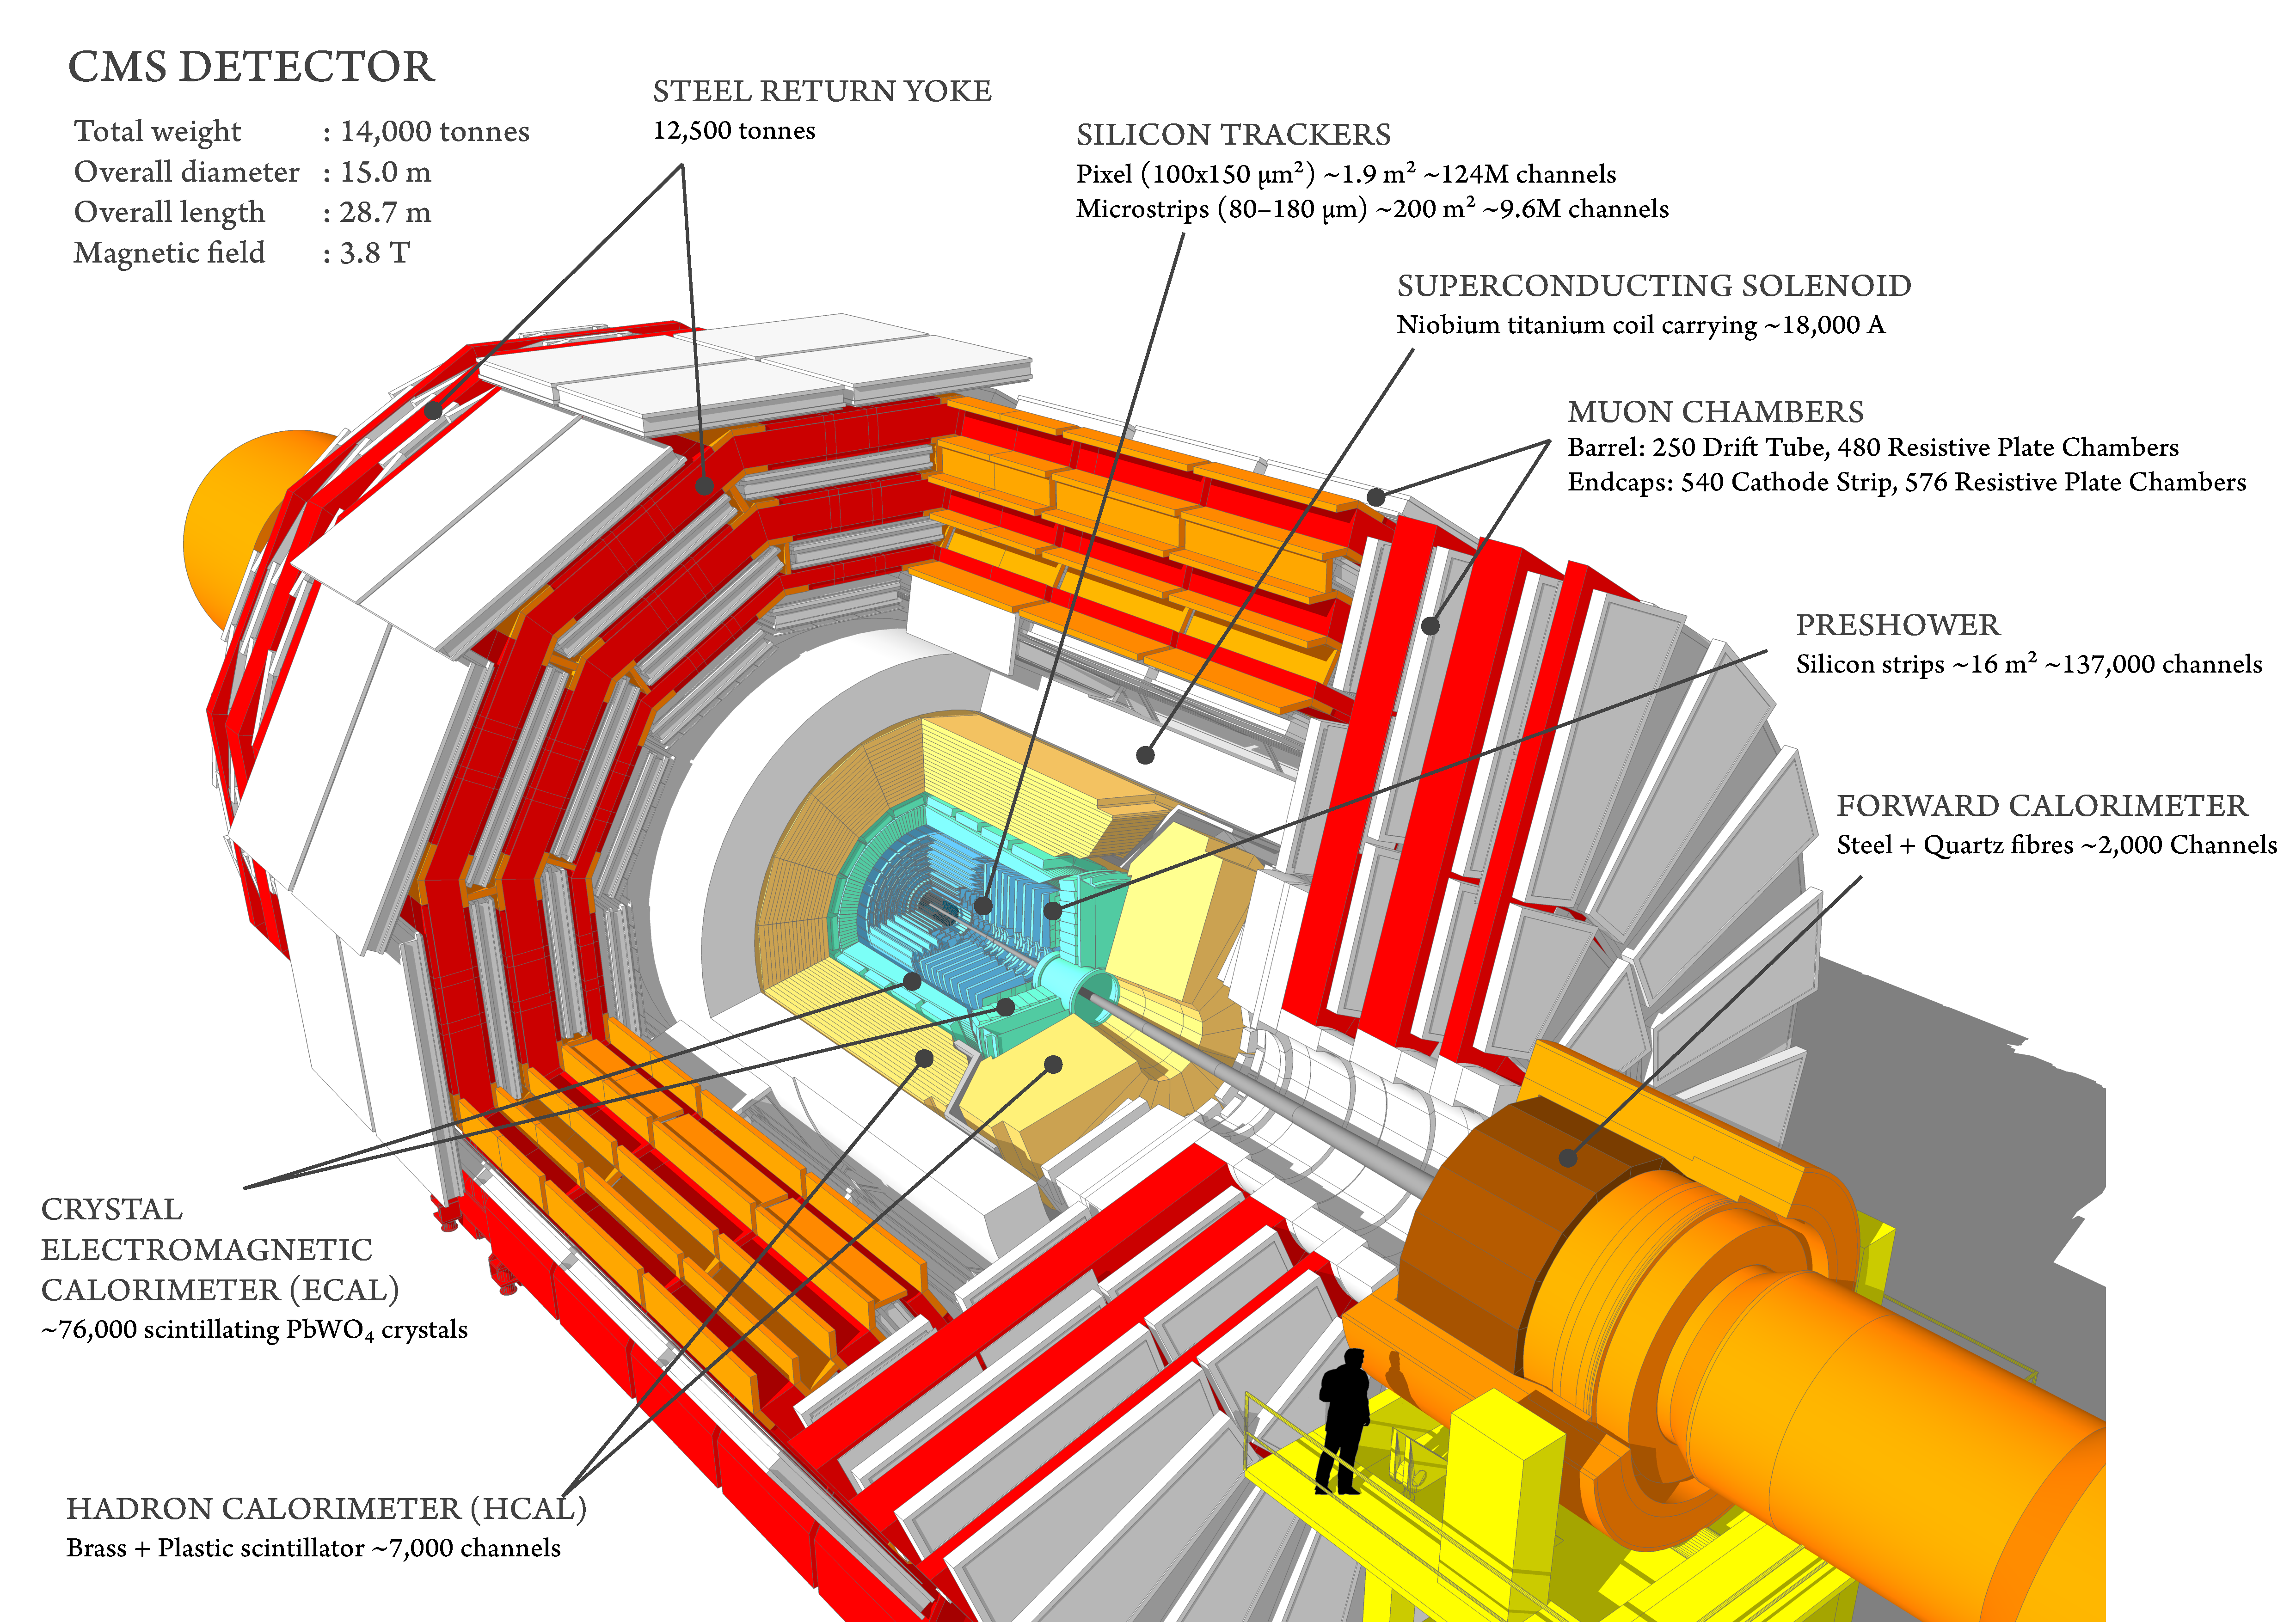
\includegraphics[width=\textwidth]{figures/cms_cutway_ME4_2.pdf}
  \caption[The CMS detector cutaway view]%
  {The CMS detector cutaway view~\cite{image-cms-cutway}}%
  \label{fig:cms-cutaway}
\end{figure}

The slice view of \gls{CMS} in Figure~\ref{fig:cms-slice}
shows how different particles leave signature in \gls{CMS} detector.
Neutral particles such photons, neutrinos, and hadrons will leave no track
in \gls{ST}, and are identified by only energy deposited or missing energy.
Electrons are identified from the track in \gls{ST} and energy deposit
in \gls{ECAL}, hadrons are heavier and they pass through \gls{ECAL}
and deposit their energy completely in \gls{HCAL}, leaving only small fraction
of energy in \gls{ECAL}.
Since muons are \gls{MIP}, they pass through whole detector with very small
fraction of energy deposit in \gls{ECAL} and \gls{HCAL}.

\begin{figure}[!ht]
  \centering
  \includegraphics[width=\textwidth]{figures/cms_slice.png}
  \caption[The CMS detector slice view]%
  {The CMS detector slice view~\cite{image-cms-slice}}%
  \label{fig:cms-slice}
\end{figure}

\subsection{
  The CMS Coordinate System
}\label{ch_cms:cms-coordinate}

CMS uses \gls{IP} of collisions as origin to define right-handed
coordinate system. The \( z \)-axis is along the beamline,
the \( x \)-axis points toward the center of the \gls{LHC},
and the \( y \)-axis points upwards, toward Earth's surface.
The transverse plane \( x - y \) is used as to calculate
most commonly used quantities like transverse momentum \( p_{T} \)
and energy \( E_{T} \).

To describe the direction of particles leaving the \gls{IP},
azimuthal \( \phi \) and polar \( \theta \) angles are used.
\( \phi \) is measured around the beam axis,
and \( \theta \) is measured from the beam axis.
In collider physics, pseudorapidity \( \eta \) (Lorentz invariant) is used
to describe direction from beam pipe instead of \( \theta \) as,

\begin{equation}
  \eta = - \ln[\tan{\theta/2}]
\end{equation}

and sometimes in terms of rapidity \( y \) as,

\begin{equation}
  y = \frac{1}{2} \ln{\frac{E+p_{z}}{E-p_{z}}}
\end{equation}

Particles kinematics can be completely described in terms of
\( p_{T} \), \( \eta \), \( \phi \), and \( E_{T} \) or mass.
The distance between the two particles \( \Delta R \) in \( \eta - \phi \) plane
is described as,

\begin{equation}
  \Delta R = \sqrt{ {(\Delta \eta)}^{2} + {(\Delta \phi)}^{2} }
\end{equation}

\subsection{
  The Superconducting Magnet
}

The superconducting magnet is the main part of the \gls{CMS} detector, it is
12.5 meters long and 6.3 meters in diameter. The magnet is cooled to
4.5\,\text{K}\xspace and 20\,\text{kA}\xspace current flows through it to
generate 3.8\Tesla{} of magnetic field with stored energy of 2.6\,\text{GJ}\xspace.

The Figure~\ref{fig:cms-magnet} shows visible superconducting magnet
and iron yoke when part of \gls{CMS} detector was lowered in the underground
cavern during installation in 2007.

The key purpose of magnet is to determine the momentum and the sign of charged
particles by bending them. The momentum resolution of the particles will
decrease with increase in \(p_T \), with constant 3.8\Tesla{} magnetic field
inside and it has momentum resolution of \(\Delta p /p \approx 10 \% \), which
is enough to determine unambiguously the sign of muons with
momentum of \(\approx 1\TeV{}/c \).

\begin{figure}[!ht]
  \centering
  \includegraphics[width=0.75\textwidth]{figures/cms_magnet_lowered.jpg}
  \caption%
  [The picture of the CMS detector central part when lowered in underground
    cavern with superconducting magnet and iron
    yoke visible]%
  {The picture of the CMS detector central part when lowered in underground
    cavern with superconducting magnet and iron
    yoke visible~\cite{image-cms-magnet}.}%
  \label{fig:cms-magnet}
\end{figure}


\subsection{
  The Tracking System
}

The \gls{CMS} tracking system \gls{ST} is the innermost part of the detector, it
is made up of pixel and strip detectors. The main goal of \gls{ST} is to
reconstruct the tracks of the charged particles with high precision in high pileup
environment.

Silicon is most commonly used material for making tracking systems because of it's
semiconductor properties, and high radiation hardness which is essential for the
innermost detector. When a p-n junction is built on silicon substrate it creates
a depletion zone with no charge carriers at the junction, and whenever
a charged particle pass through the depletion zone it creates a electron-hole pair,
and under reverse bias this electron-hole generates electrical signal. The \gls{CMS}
tracking consists of about 124 million channels of such junctions in
pixel detector and 10 million in strip detector.

The pixel detector was upgraded in 2017 and the comparison of layers before
and after the upgrade is shown in Figure~\ref{fig:cms-pixel}. It is made up of
four barrel layers and three endcaps, with nearest barrel layer being 3\cm{}
away from beamline for precise measurement of \gls{IP}.
Because of the large number of pixel channels, the readout is done by \glspl{ASIC}.

The outermost part of \gls{ST} detector is made of silicon strips. It allows large
coverage by reducing number of readout channels. It has 10 layers in barrel region
and 12 discs in endcap region. For better signal-to-noise ratio and radiation
tolerance both pixel and strip operates at -20\,\de\text{C}\xspace.

\begin{figure}[!ht]
  \centering
  \begin{minipage}[c]{.62\textwidth}
    \includegraphics[trim={80pt 0 80pt 0},clip,width=\textwidth]%
    {figures/cms_pixel_phase1.pdf}
  \end{minipage}
  \begin{minipage}[c]{.35\textwidth}
    \includegraphics[width=\textwidth]{figures/cms_pixel_phase1_04.png}
  \end{minipage}
  \caption[The CMS pixel upgrade]%
  {The CMS pixel upgrade. The left is cross sectional view of pixel detector
    layers before upgrade (bottom) and after Phase 1 upgrade (top).
    The right is view pixel barrel before upgrade (left)
    and after upgrade (right)~\cite{image-cms-pixel}.}%
  \label{fig:cms-pixel}
\end{figure}

\subsection{
  The Electromagnetic Calorimeter
}

\subsection{
  The Hadronic Calorimeter
}

\subsection{
  The Trigger System
}

\section{
  High Granularity Calorimeter Upgrade
 }

About \gls{HGCAL} Upgrade
